\documentclass[
% -- opções da classe memoir --
12pt,				% tamanho da fonte
openright,			% capítulos começam em pág ímpar (insere página vazia caso preciso)
oneside,			% para impressão em recto e verso. Oposto a oneside
a4paper,			% tamanho do papel. 
% -- opções da classe abntex2 --
%chapter=TITLE,		% títulos de capítulos convertidos em letras maiúsculas
%section=TITLE,		% títulos de seções convertidos em letras maiúsculas
%subsection=TITLE,	% títulos de subseções convertidos em letras maiúsculas
%subsubsection=TITLE,% títulos de subsubseções convertidos em letras maiúsculas
% -- opções do pacote babel --
english,			% idioma adicional para hifenização
brazil				% o último idioma é o principal do documento
]{abntex2}

% ---
% Pacotes acrescentados
% ---
%\usepackage[portuguese, ruled, linesnumbered]{algorithm2e}
%\usepackage{algorithmic}

% ---
% Pacotes básicos 
% ---
\usepackage{lmodern}			% Usa a fonte Latin Modern			
\usepackage[T1]{fontenc}		% Selecao de codigos de fonte.
\usepackage[utf8]{inputenc}		% Codificacao do documento (conversão automática dos acentos)
\usepackage{lastpage}			% Usado pela Ficha catalográfica
\usepackage{indentfirst}		% Indenta o primeiro parágrafo de cada seção.
\usepackage{color}				% Controle das cores
\usepackage{url}				% Citar URLs
\usepackage{graphicx}			% Inclusão de gráficos
\usepackage{microtype} 			% para melhorias de justificação
\usepackage{booktabs}
\usepackage{multirow}
\usepackage[table]{xcolor}
\setlength{\aboverulesep}{0pt}
\setlength{\belowrulesep}{0pt}
\usepackage{scalefnt}
\usepackage{pdfpages}
% ---

% ---
% Pacotes adicionais, usados apenas no âmbito do Modelo Canônico do abnteX2
% ---
\usepackage{lipsum}				% para geração de dummy text
\usepackage{amssymb}			% para uso de símbolos matemáticos
% ---

% ---
% Pacotes de citações
% ---
\usepackage[brazilian,hyperpageref]{backref}	 % Paginas com as citações na bibl
\usepackage[alf]{abntex2cite}	% Citações padrão ABNT


% Pacotes adicionais Wal
\usepackage{subfig}  %para exibir figuras lado a lado
\usepackage{listings} % Para inclusao de codigos fontes
\usepackage{color}
\definecolor{mygreen}{rgb}{0,0.6,0}
\definecolor{mygray}{rgb}{0.5,0.5,0.5}
\definecolor{mymauve}{rgb}{0.58,0,0.82}
\lstset{ %
	backgroundcolor=\color{white},   % choose the background color; you must add \usepackage{color} or \usepackage{xcolor}
	basicstyle=\footnotesize,        % the size of the fonts that are used for the code
	breakatwhitespace=false,         % sets if automatic breaks should only happen at whitespace
	breaklines=true,                 % sets automatic line breaking
	captionpos=t,                    % sets the caption-position to bottom
	commentstyle=\color{mygreen},    % comment style
	deletekeywords={...},            % if you want to delete keywords from the given language
	escapeinside={\%*}{*)},          % if you want to add LaTeX within your code
	extendedchars=true,              % lets you use non-ASCII characters; for 8-bits encodings only, does not work with UTF-8
	frame=single,	                 % adds a frame around the code
	keepspaces=true,                 % keeps spaces in text, useful for keeping indentation of code (possibly needs columns=flexible)
	keywordstyle=\color{blue},       % keyword style
	language=Octave,                 % the language of the code
	otherkeywords={*,...},           % if you want to add more keywords to the set
	numbers=left,                    % where to put the line-numbers; possible values are (none, left, right)
	numbersep=5pt,                   % how far the line-numbers are from the code
	numberstyle=\tiny\color{mygray}, % the style that is used for the line-numbers
	rulecolor=\color{black},         % if not set, the frame-color may be changed on line-breaks within not-black text (e.g. comments (green here))
	showspaces=false,                % show spaces everywhere adding particular underscores; it overrides 'showstringspaces'
	showstringspaces=false,          % underline spaces within strings only
	showtabs=false,                  % show tabs within strings adding particular underscores
	stepnumber=1,                    % the step between two line-numbers. If it's 1, each line will be numbered
	stringstyle=\color{mymauve},     % string literal style
	tabsize=2,	                   	 % sets default tabsize to 2 spaces
	title=\lstname,                  % show the filename of files included with \lstinputlisting; also try caption instead of title
	numberbychapter=false
}


% --- 
% CONFIGURAÇÕES DE PACOTES
% --- 

\hyphenation{a-di-cio-nal-men-te}

% ---
% Configurações do pacote backref
% Usado sem a opção hyperpageref de backref
\renewcommand{\backrefpagesname}{Citado na(s) página(s):~}
% Texto padrão antes do número das páginas
\renewcommand{\backref}{}
% Define os textos da citação
\renewcommand*{\backrefalt}[4]{
	\ifcase #1 %
	Nenhuma citação no texto.%
	\or
	Citado na página #2.%
	\else
	Citado #1 vezes nas páginas #2.%
	\fi}%
% ---

%-----
%Adaptações do formato ABNT para UNESP
\addto\captionsbrazil{
	\renewcommand{\listfigurename}{Lista de Figuras}
	\renewcommand{\listtablename}{Lista de Tabelas}
	\renewcommand{\listadesiglasname}{Lista de Abreviaturas e Siglas}
	%\renewcommand{\folhadeaprovacaoname}{Folha de Aprovação}
	\renewcommand{\listadesimbolosname}{Lista de Símbolos}
}
%-----


% ---
% Informações de dados para CAPA e FOLHA DE ROSTO
% ---
\uppercase{\titulo{Trabalho de Classificação}}
\autor{Maicon Dall'Agnol}
\local{Rio Claro - SP}
\data{2019}
\orientador[Professora:]{Profa. Dra. Adriane Beatriz de Souza Serapião}
\instituicao{%
	UNIVERSIDADE ESTADUAL PAULISTA
	\par
	``J\'ULIO DE MESQUITA FILHO''
	\par
	Instituto de Geociências e Ciências Exatas - IGCE
	\par
	Curso de Bacharelado em Ciências da Computação}

\tipotrabalho{Trabalho de graduação}
% O preambulo deve conter o tipo do trabalho, o objetivo, 
% o nome da instituição e a área de concentração 
\preambulo{Trabalho de graduação da disciplica Tópico de Aprendizado de Máquina pelo Curso de Bacharelado em Ciências da Computação do Instituto de Geociências e Ciências Exatas da Universidade Estadual Paulista “Júlio de Mesquita Filho”, Câmpus de Rio Claro. }
% ---

% ---
% Configurações de aparência do PDF final

% alterando o aspecto da cor azul
\definecolor{blue}{RGB}{41,5,195}

% informações do PDF
\makeatletter
\hypersetup{
	%pagebackref=true,
	pdftitle={\@title}, 
	pdfauthor={\@author},
	pdfsubject={\imprimirpreambulo},
	pdfcreator={regras de associação},
	pdfkeywords={java}{proposta de trabalho}{unesp}, 
	colorlinks=false,       		% false: boxed links; true: colored links
	linkcolor=blue,          	% color of internal links
	citecolor=blue,        		% color of links to bibliography
	filecolor=magenta,      		% color of file links
	urlcolor=blue,
	bookmarksdepth=4
}
\makeatother
% --- 

% --- 
% Espaçamentos entre linhas e parágrafos 
% --- 

% O tamanho do parágrafo é dado por:
\setlength{\parindent}{1.3cm}

% Controle do espaçamento entre um parágrafo e outro:
\setlength{\parskip}{0.2cm}  % tente também \onelineskip

% ---
% compila o indice
% ---
\makeindex
% ---

% ----
% Início do documento
% ----
\begin{document}
	
	% Seleciona o idioma do documento (conforme pacotes do babel)
	%\selectlanguage{english}
	\selectlanguage{brazil}
	
	% Retira espaço extra obsoleto entre as frases.
	\frenchspacing 
	
	% ----------------------------------------------------------
	% ELEMENTOS PRÉ-TEXTUAIS
	% ----------------------------------------------------------
	
	\pretextual
	
 	  \begin{capa}
	\begin{center}
	\Large\imprimirinstituicao
	\end{center}

	\begin{center}
	\vspace*{3.4cm}
	\Large MAICON DALL'AGNOL
	\vspace*{1.5cm}
	
	\Large \textbf{\imprimirtitulo}
	
	\vspace*{3.4cm}
	
	\noindent Professor: Dr. Ivan Rizzo Guilherme
	
	\vspace*{3.4cm}
	
	{\large\imprimirlocal}
	\par
	{\large\imprimirdata}
	\vspace*{1cm}
	\end{center}
  \end{capa}
	
	%\begin{folhaderosto}
	\begin{center}		
		
		\vspace*{\fill}\vspace*{\fill}
		\begin{center}
			\ABNTEXchapterfont\bfseries\Large\imprimirtitulo
		\end{center}
		\vspace*{\fill}
		
		\hspace{.45\textwidth}
		\begin{minipage}{.5\textwidth}
			\SingleSpacing
			\imprimirpreambulo
		\end{minipage}%		
		
		\vspace*{1cm}
		\begin{flushright}
			\noindent Aluno: Maicon Dall'Agnol
		\end{flushright}
		\vspace*{1cm}
		\begin{flushright}
			\noindent Professora: Dra. Adriane Beatriz de Souza Serapião
		\end{flushright}
		\vspace*{1cm}
				
				
		{\large\imprimirlocal}
		\par
		{\large\imprimirdata}
		\vspace*{1cm}
		
	\end{center}
\end{folhaderosto}
	
	%\include{errata}
	
	%\include{folhadeaprovacao}
	
	%\include{dedicatoria}
	
	%\include{agradecimentos}
	
	%\include{epigrafe}
	
	%\setlength{\absparsep}{18pt} % ajusta o espaçamento dos parágrafos do resumo
	%\include{resumo}
	
	%
%\pdfbookmark[0]{\listfigurename}{lof}
%\listoffigures*
%\cleardoublepage
% ---

% ---
% inserir lista de tabelas
% ---
%\pdfbookmark[0]{\listtablename}{lot}
%\listoftables*
%\cleardoublepage
% ---

% ---
% inserir lista de algoritmos
% ---
%\pdfbookmark[0]{Lista de Algoritmos}{loa}
%\listofalgorithms
%\cleardoublepage
% ---

% ---
% Lista de scripts
% ---
%\pdfbookmark[0]{Lista de Scripts}{loa}
%\lstlistoflistings
%\cleardoublepage

% ---
% inserir lista de abreviaturas e siglas
% ---
%\begin{siglas}
%	\item[KDD] Knowledge Discovery in Databases
%	\item[MD] Mineração da Dados
%	\item[MO] Medida Objetiva
%	\item[RA] Regra de Associação
%\end{siglas}
% ---

%\newpage
%\listofalgorithms*       % Lista de algoritmos
%\addcontentsline{toc}{section}{Lista de Algoritmos}

% ---
% inserir o sumario
% ---
\pdfbookmark[0]{\contentsname}{toc}
\tableofcontents*
\cleardoublepage
% ---

	
	% ----------------------------------------------------------
	% ELEMENTOS TEXTUAIS
	% ----------------------------------------------------------
	\textual
	
	%Capitulos
	\chapter{Introdução}\label{cap_intro}

Este trabalho consiste em aplicar o conhecimento de Classificadores adquirido na disciplina Tópicos: Aprendizado de Máquina. Tem-se como objetivo:

\begin{itemize}
\item Escolha dois datasets rotulados.
\item Realize a análise estatística, visualização e pré-processamento dos dados.
\item Realize os experimentos criando duas bases de teste distintas:
\begin{itemize}
\item considerando todos os atributos do dataset;
\item selecionando alguns atributos e descartando outros.
\end{itemize}
\item Aplique três métodos de classificação distintos nas duas bases acima referentes a cada dataset.
\item Para cada dataset, em cada uma das bases, analise os resultados segundo medidas de qualidade de classificação, usando índices de validação externa (acurácia, recall, precisão, F-measure, índice Kappa) e cruva ROC.
\item Proponha uma maneira adicional de comparar os resultados obtidos além das medidas acima.
\item Compare e interprete os resultados dos dois experimentos em cada dataset.
\item Faça tabela com as medidas de validação	
\end{itemize}

	\chapter{Desenvolvimento}\label{cap_desenv}

Para o desenvolvimento das atividades inicialmente foram escolhidos duas bases bases de dados. A primeira base a ser utilizada corresponde a dados de uma central elétrica de ciclo combinado ao longo de 6 anos tendo informações como temperatura, pressão ambiente, umidade, vácuo de exaustão e saída de energia elétrica horária líquida, sendo este ultimo o escolhido para ser predito; A segunda base é composta do histórico de tempo de 2006 a 2016 em Szeged, Hungria, contendo hora, temperatura, umidade, entre outros atributos, sendo a temperatura escolhida como atributo a ser predito.

\section{Pré-processamento e Visualização}
Para ambos \textit{datasets} utilizou-se de um biblioteca do Python chamada Pandas Profiling que descreve e faz uma pré análise dos \textit{datasets}, como linhas duplicadas, dados faltantes, grande variância entre os dados.

A partir desta análise notou-se que no dataset do tempo há duas variáveis com alta correlação, portanto retirou-se uma delas. Também na segunda base, há diversos atributos categóricos que foram removidos a fim de agilizar o treinamento dos algoritmos (também diminuiu-se o dataset de mais 94000 para 10000), visto que o tempo de treinamento dos algoritmos é longo.

Em ambas visualizações dos \textit{datasets} é possivel notar uma certa linearidade entre os atributos PE e AT, para o primeiro dataset, e Humidity e Temperature, no segundo, deste modo, escolheu-se esses atributos para serem usados na visualização dos itens preditos e reais.

Para aplicação dos algoritmos de regressão os dados foram escalonados utilizando o StandardScaler.

Para separação de treino e teste utilizou-se uma divisão de $20\%$ para teste e $80\%$ para treino, de forma aleatória.

\section{Regressão}

Na aplicação dos algoritmos de regressão foram utilizados os algoritmos de regressão linear, regressão polinomial, SVR, utilizando os kernels linear, sigmoide, RBF e polinomial, rede neural MLP. Alguns algoritmos tiveram seus parâmetros \textit{default} alterados para outros valores, os demais permanecem inalterados.


\section{Avaliação}

Os resultados foram medidos para os dados de treino e de teste de ambas bases. Para a primeira base a Tabela~\ref{ceteste} corresponde aos resultados da base de teste e a Tabela~\ref{cetreino}, aos dados de treino.

\begin{table}[h]
	\centering
	\begin{tabular}{|l|l|l|l|l|}
		\hline
		Algoritmo                & EQM    & $R^2$     & REQM   & SEQ        \\ \hline
		Regressão Linear - Teste & 0,068  & 0,932  & 0,261  & 130,01     \\ \hline
		SVR - RBF - Teste        & 0,054  & 0,946  & 0,231  & 102,41     \\ \hline
		SVR - Linear - Teste     & 0,068  & 0,932  & 0,261  & 130,454    \\ \hline
		SVR - Sigmoide - Teste   & 298,19 & -0,027 & 17,268 & 570735,341 \\ \hline
		SVR - Polinomial - Teste & 0,212  & 0,787  & 0,461  & 406,592    \\ \hline
		MLP - Teste              & 0,053  & 0,946  & 0,231  & 102,359    \\ \hline
	\end{tabular}
	\caption{Avaliação dos dados de teste da central elétrica.}
\label{ceteste}
\end{table}


\begin{table}[h]
	\centering
	\begin{tabular}{|l|l|l|l|l|}
		\hline
		Algoritmo                 & EQM     & $R^2$     & REQM   & SEQ         \\ \hline
		Regressão Linear - Treino & 0,072   & 0,928  & 0,269  & 552,272     \\ \hline
		SVR - RBF - Treino        & 0,054   & 0,946  & 0,233  & 415,487     \\ \hline
		SVR - Linear - Treino     & 0,073   & 0,927  & 0,269  & 555,226     \\ \hline
		SVR - Sigmoide - Treino   & 299,318 & -0,027 & 17,301 & 2290976,223 \\ \hline
		SVR - Polinomial - Treino & 0,219   & 0,781  & 0,468  & 1675,504    \\ \hline
		MLP - Treino              & 0,054   & 0,946  & 0,233  & 416,689     \\ \hline
	\end{tabular}
	\caption{Avaliação dos dados de treino da central elétrica.}
	\label{cetreino}
\end{table}

Comparando as medidas para todos os algoritmos aplicados ao dataset da central elétrica é possível observar que todos, exceto o SVR - Sigmoide, apresentam bons resultados em ambas bases, ficando bem próximos aos valores reais, isto é demonstrado pelo baixo valor de EQM e alto $R^2$, por exemplo.

\begin{table}[h]
	\begin{tabular}{|l|l|l|l|l|}
		\hline
		Algoritmo                & EQM       & $R^2$         & REQM    & SEQ           \\ \hline
		Regressão Linear - Teste & 0,593     & 0,406      & 0,77    & 1185,398      \\ \hline
		SVR - RBF - Teste        & 0,6       & 0,399      & 0,774   & 1199,215      \\ \hline
		SVR - Linear - Teste     & 0,601     & 0,397      & 0,775   & 1202,513      \\ \hline
		SVR - Sigmoide - Teste   & 51226,694 & -51370,514 & 226,333 & 102453388,722 \\ \hline
		SVR - Polinomial - Teste & 0,698     & 0,3        & 0,835   & 1395,272      \\ \hline
		MLP - Teste              & 0,583     & 0,415      & 0,764   & 1166,166      \\ \hline
	\end{tabular}
	\caption{Avaliação dos dados de teste do tempo.}
	\label{tempoteste}
\centering
\end{table}

\begin{table}[h]
	\begin{tabular}{|l|l|l|l|l|}
		\hline
		Algoritmo                 & EQM       & $R^2$         & REQM    & SEQ           \\ \hline
		Regressão Linear - Treino & 0,585     & 0,416      & 0,765   & 4677,922      \\ \hline
		SVR - RBF - Treino        & 0,577     & 0,423      & 0,76    & 4618,342      \\ \hline
		SVR - Linear - Treino     & 0,592     & 0,408      & 0,769   & 4736,851      \\ \hline
		SVR - Sigmoide - Treino   & 52816,201 & -52785,446 & 229,818 & 422529610,722 \\ \hline
		SVR - Polinomial - Treino & 0,755     & 0,245      & 0,869   & 6040,982      \\ \hline
		MLP - Treino              & 0,575     & 0,425      & 0,758   & 4599,792      \\ \hline
	\end{tabular}
	\caption{Avaliação dos dados de treino do tempo.}
	\label{tempotreino}
	\centering
\end{table}

Avaliando os resultados obtidos para o dataset do tempo, presentes nas Tabelas~\ref{tempoteste} e \ref{tempotreino}, de teste e treino, respectivamente, é possivel concluir que o mesmo não ocorre aqui, apresentando dados mais esparsos, tendo todas as medidas mais elevados, contudo ainda sim apresentam baixos valores de EQM e médio $R^2$.

Olhando para os resultado nas bases de teste e treino, para a primeira base de dados os algoritmos MLP e SVR - RBF apresentaram resultados bem próximos, com uma ligeira vantagem para o MLP. Na segunda base os algoritmos MLP e Regressão Linear tiveram também resultados muito próximos, novamente com uma pequena vantagem para o MLP. Portanto, em termos gerais para os dois \textit{datasets} o MLP se saiu melhor.

	%\chapter{Conclusão}\label{cap_conclu}

Aqui vai a conclusão
	
	
	% ----------------------------------------------------------
	% Finaliza a parte no bookmark do PDF
	% para que se inicie o bookmark na raiz
	% e adiciona espaço de parte no Sumário
	% ----------------------------------------------------------
	\phantompart
	
	%\chapter{Conclusão}
	
	
	% ----------------------------------------------------------
	% ELEMENTOS PÓS-TEXTUAIS
	% ----------------------------------------------------------
	\postextual
	% ----------------------------------------------------------
	
	% ----------------------------------------------------------
	% Referências bibliográficas
	% ----------------------------------------------------------
	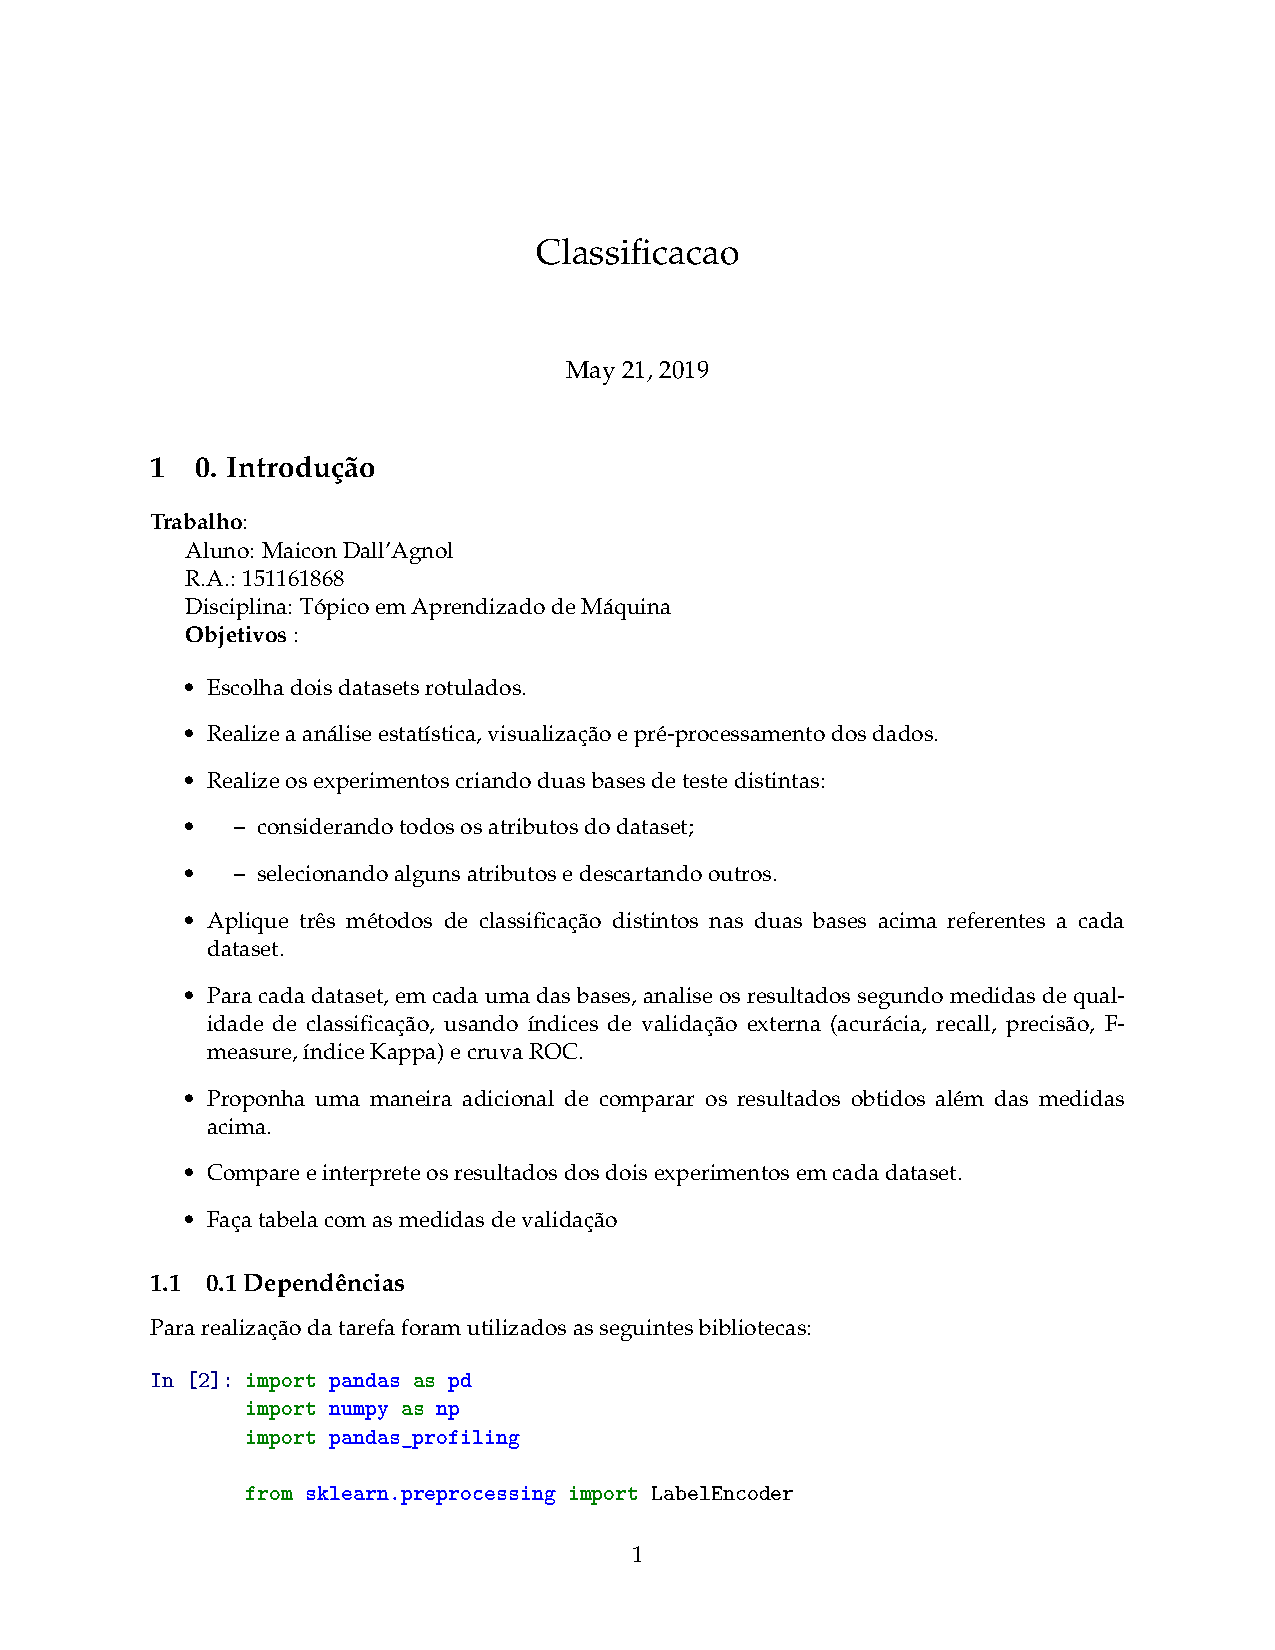
\includepdf[page=-]{Classificacao}
	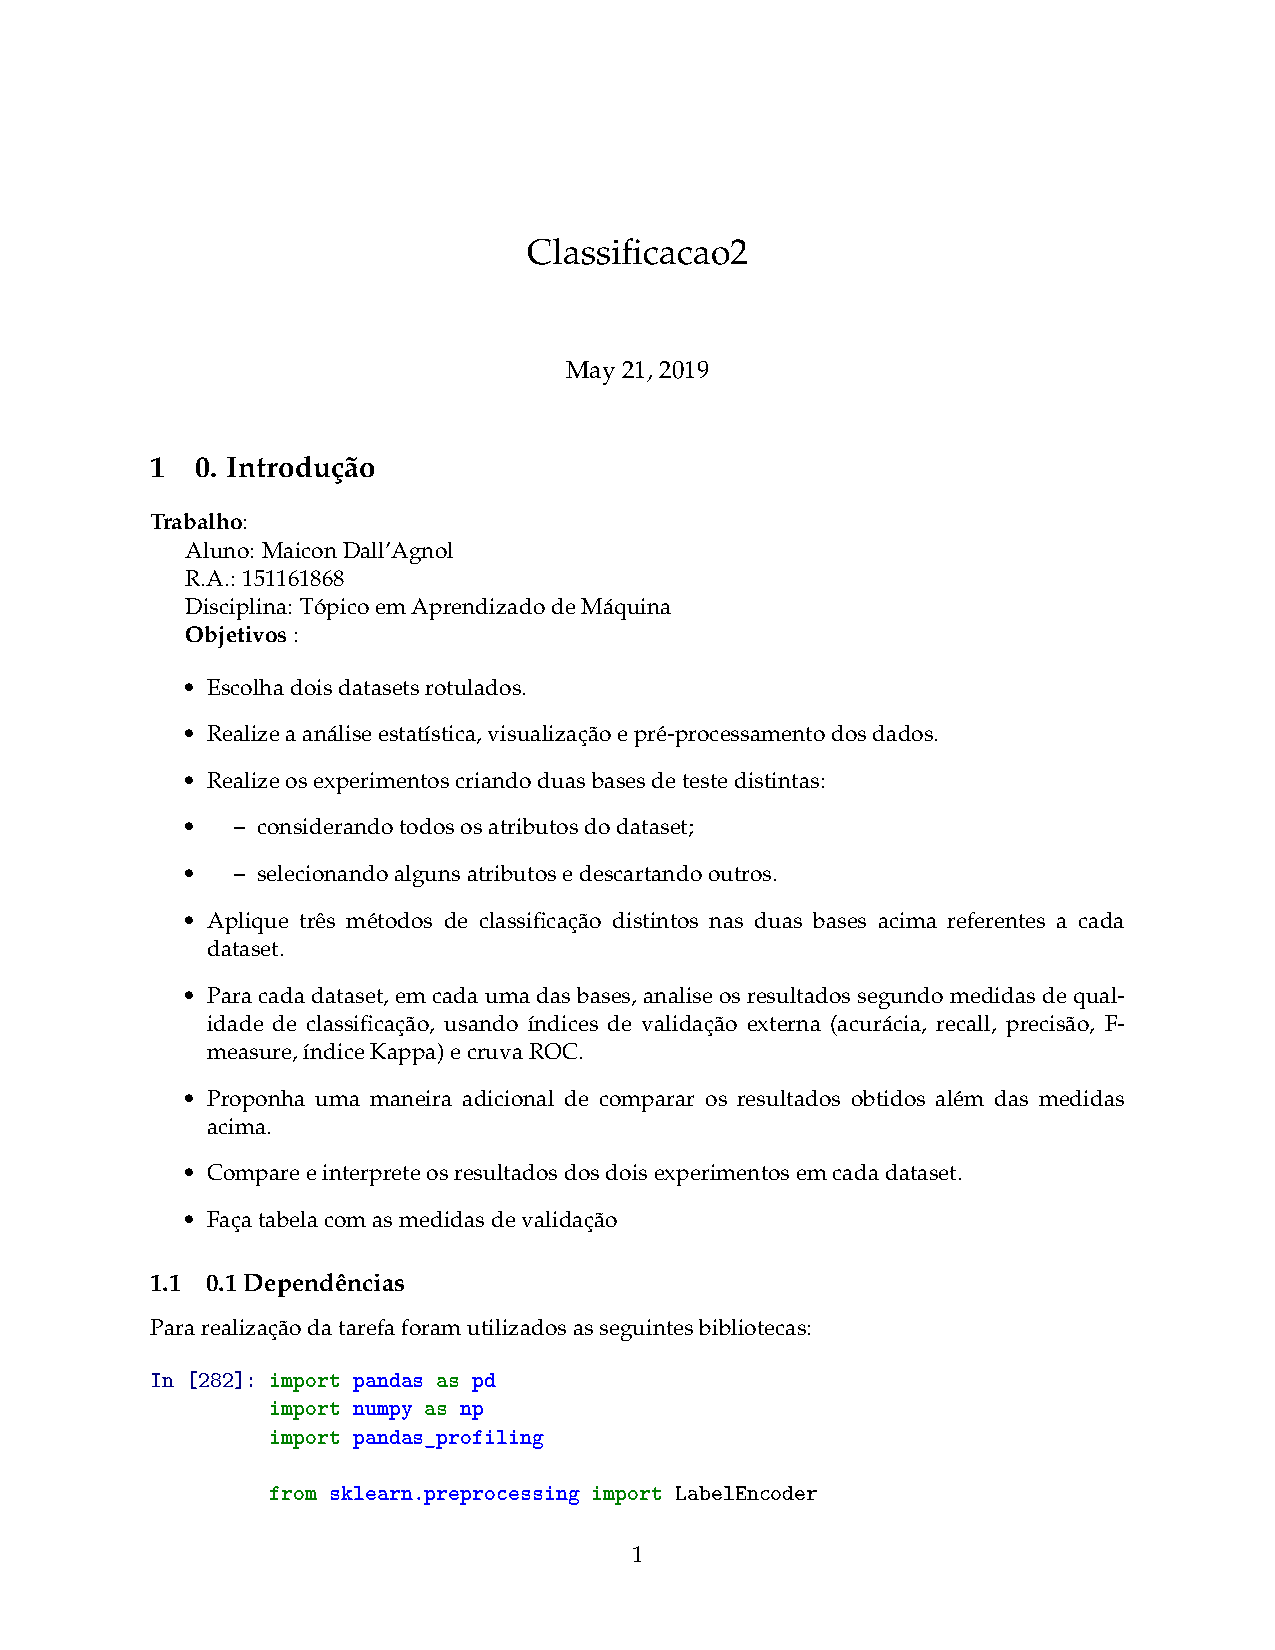
\includepdf[page=-]{Classificacao2}
	
		\bibliography{references}
\end{document}
